\section{Background Theory}
In order to identify the best means of gaining navigation for \gls{tiberius3}, an understanding of the key areas needed to be obtained via some research into the background of navigation techniques.
\subsection{GPS}

\begin{figure}[!htb]
\begin{center}
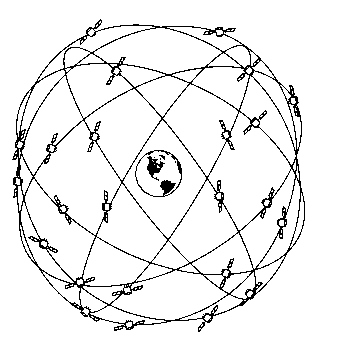
\includegraphics[width=10cm]{GPS.jpg}
\end{center}
\caption{\gls{GPS} satellites around the world\cite{RobotNavigation}}
\label{fig:AGNavigation}
\end{figure}

\gls{GPS} is a key component of the outdoor navigation systems. It was developed by the United States Air and Navel forces in the 1970s and is now used within a wide range of tracking devices. \gls{GPS} relies on a series of satellites positioned in orbit around the world, as well as stations on earth. These things combined create a system that lets users find there latitude and longitude position with a high degree of accuracy.
\subsection{Path Planning}
For \gls{tiberius3} to be able to navigate through an area, some form of path planning was required. This meant that an understanding of different methods that create paths through terrain was needed to build one for the project.

\begin{itemize}
\item \textbf{A-Star}, is an algorithm that operates on a grid area that has been pre-built around the robot that needs to move. This algorithm gives each square of a grid a heuristic value as well as a cost value that determine the effect that travelling to that square from the robot's current location would entail. It provides an efficient and accurate path for a robot to follow, provided that the data within the grid is correct.
\item \textbf{D-Star}, makes assumptions about the areas of the grid that there is little data about and creates a path using these assumptions. As more data is found the path is re-calculated to account for the new data.
\item \textbf{AD-Star}, or dynamic A-Star, is a dynamic version of the A-Star algorithm that continuously improves its path as new data comes in. This means that there is a lot more compilation but with the benefit of not wasting movement by travelling in an inefficient manner.
\end{itemize}
The chosen path planning algorithm is based on the A-Star algorithm but has elements of AD-Star where it re-plans if an obstacle is found on the path or if the path does not lead to the final destination.

\subsection{SLAM}
\gls{SLAM} is an algorithm that creates and updates a map of an environment that was unknown before the beginning of the algorithm. It also tries to find the location of the robot within the given environment using the algorithm. Traditionally \gls{SLAM} is achieved by using sensors such as a \gls{LIDAR}, of which there is one on \gls{tiberius3}.